
\chapter{SOLUTION}
\label{ch:Solution}

\section{Overview}

We propose the Onion Name System (OnioNS) as an abstraction layer to hidden service addresses and introduce ``.tor'' as a new pseudo-TLD for this purpose. The system has three main aspects: the generation of self-signed claims on domain names by hidden service operators, the processing of domain information within the OnioNS servers, and the receiving and authentication of domain names by a Tor client.

First, a hidden service operator, Bob, generates an association between a meaningful second-level domain name and his .onion address. Without loss of generality, let this be ``example.tor $ \rightarrow $ onions55e7yam27n.onion''. We introduce a proof-of-work scheme that requires Bob to expend computational and memory resources to claim ``example.tor'', a more privacy-enhanced alternative to financial compensation to a central authority. Proof-of-work systems are noteworthy for their asymmetry: they require the issuer to spend effort to find an answer to a moderately hard computational problem, but once solved can be easily verified correct by any recipient. The requirement of proof-of-work fulfils three main purposes:

\begin{enumerate}
	\item Significantly reduces the threat of DoS flood attack.
	\item Introduces a barrier-of-entry that encourages the utilization of domain names and the availability of the underlying hidden services.
	\item Increases the difficulty of domain squatting, a denial-of-service attack where a third-party claims one or more valuable domain names for the purpose of denying or selling them en masse to others.
\end{enumerate}

Second, Bob uses a Tor circuit to anonymously transmit his Record to an authoritative short-lived random subset of OnioNS servers, known as the \emph{Quorum}, inside the Tor network. The Quorum archive Bob's Record in a sequential public ledger known as a \emph{Pagechain}, of which each OnioNS node holds their own local copy. Bob's Record is received by all Quorum nodes and share signatures of their knowledge with each other, so they maintain a common database.

Third, Alice, uses a Tor client to anonymously connect to a name server outside the Quorum but mirroring their database, then ask for ``example.tor''. Alice receives Bob's Record, verifies it signature and proof-of-work, and follows the association to ``onions55e7yam27n.onion''. As Bob's Record is self-signed using Bob's private key, Alice can verify the Record's authenticity. Finally, Alice uses this address and the Tor hidden service protocol to contact Bob. In this way, Alice can contact Bob through his chosen domain name without resorting to use lower-level hidden service addresses. The uniqueness and authenticity of the Bob's domain name is maintained by the subset of Tor nodes.

\section{Definitions}

To discuss OnioNS precisely we must first define some central terms that we will use throughout the rest of this document. We detail their exact contents in section \ref{sec:DataStructures} and how they are used throughout sections \ref{sec:BasicDesign} and \ref{sec:Protocols}.

\textbf{domain name} is a case-insensitive identification string claimed by a hidden service operator. The syntax of OnioNS domain names mirrors the Internet DNS; we use a sequence of name-delimiter pairs with a .tor pseudo top-level domain (TLD) that is not used on the Internet DNS. The TLD is a name at depth one and is preceded by names at sequentially increasing depth. The term ``domain name'' refers to the identification string as a whole, while ``second-level domain'' refers to the central name that is immediately followed by the TLD, as illustrated in Figure \ref{fig:sampleDomain}. Domain names point to \emph{destinations} -- other domain names with either the .tor or .onion TLD.

		\begin{figure}[htbp]
			\centering
			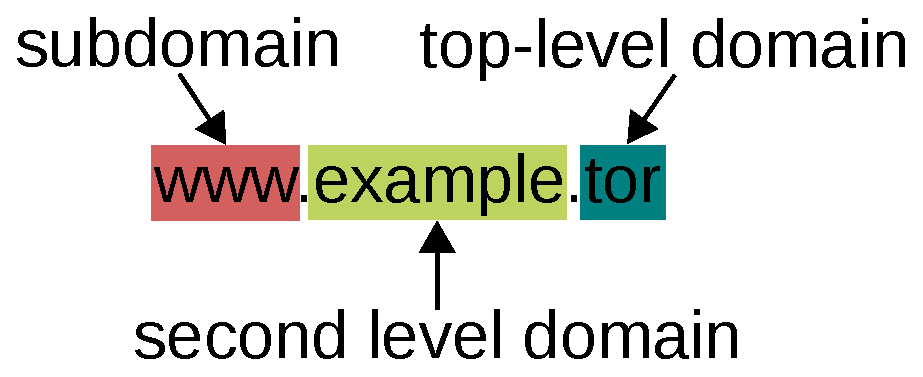
\includegraphics[width=0.5\textwidth]{images/domain-name.eps}
			\caption{A sample domain name: a sequence of labels separated by delimiters. In OnioNS, hidden service operators build associations between second-level domain names and their hidden service address.}
			\label{fig:sampleDomain}
		\end{figure}

	The Internet DNS defines a hierarchy of administrative realms that are closely tied to the depth of each name. By contrast, OnioNS makes no such distinction; we let hidden service operators claim a second-level name and then control all names of greater depth under that second-level name.

A \textbf{Record} is a small textual data structure that contains a single second-level domain name, a mapping of subdomains to .tor or .onion pseudo-TLD destinations, proof-of-work, a digital signature, a public key, and an optional PGP fingerprint. Records are issued by hidden service operators and sent to OnioNS servers. Every Record is self-signed with the hidden service's key. In section \ref{sec:Record} we describe the five different types of Records: Create, Modify, Move, Renew, and Delete.

A \textbf{Page} is textual database designed to archive one or more Records in long-term storage. Pages are held and digitally signed by OnioNS nodes and are writable only for fixed periods of time before they are read-only. Each Page contains a link to a previous Page, forming an append-only public ledger known as an \emph{Pagechain}. This forms a two dimensional distributed data structure: the chain of Pages grows over time and there are multiple redundant copies of each Page spread out across the network at any given time.
		
A \textbf{Mirror} is any machine (inside or outside of the Tor network) that has performed a synchronization (section \ref{sec:Synchronization}) against the OnioNS network and now holds a complete copy of the Pagechain. Mirrors do not actively participate in the OnioNS network and do not have the power to manipulate the main page-chain.

A \textbf{Quorum Candidates} are \emph{Mirrors} inside the Tor network that have also fulfilled two additional requirements: 1) they must demonstrate that they are an up-to-date Mirror, and 2) that they have sufficient CPU and bandwidth capabilities to handle powering OnioNS in addition to their regular Tor duties. In other words, they are qualified and capable to power OnioNS, but have not yet been chosen to do so.

The \textbf{Quorum} is a subset of Quorum Candidates who have active responsibility over maintaining the master OnioNS Pagechain. Each Quorum node actively its own Page, which has a lifetime of that Quorum. The Quorum is randomly chosen from Quorum Candidates as described in section \ref{sec:ProtoTorClients}.

\begin{figure}[htbp]
	\centering
	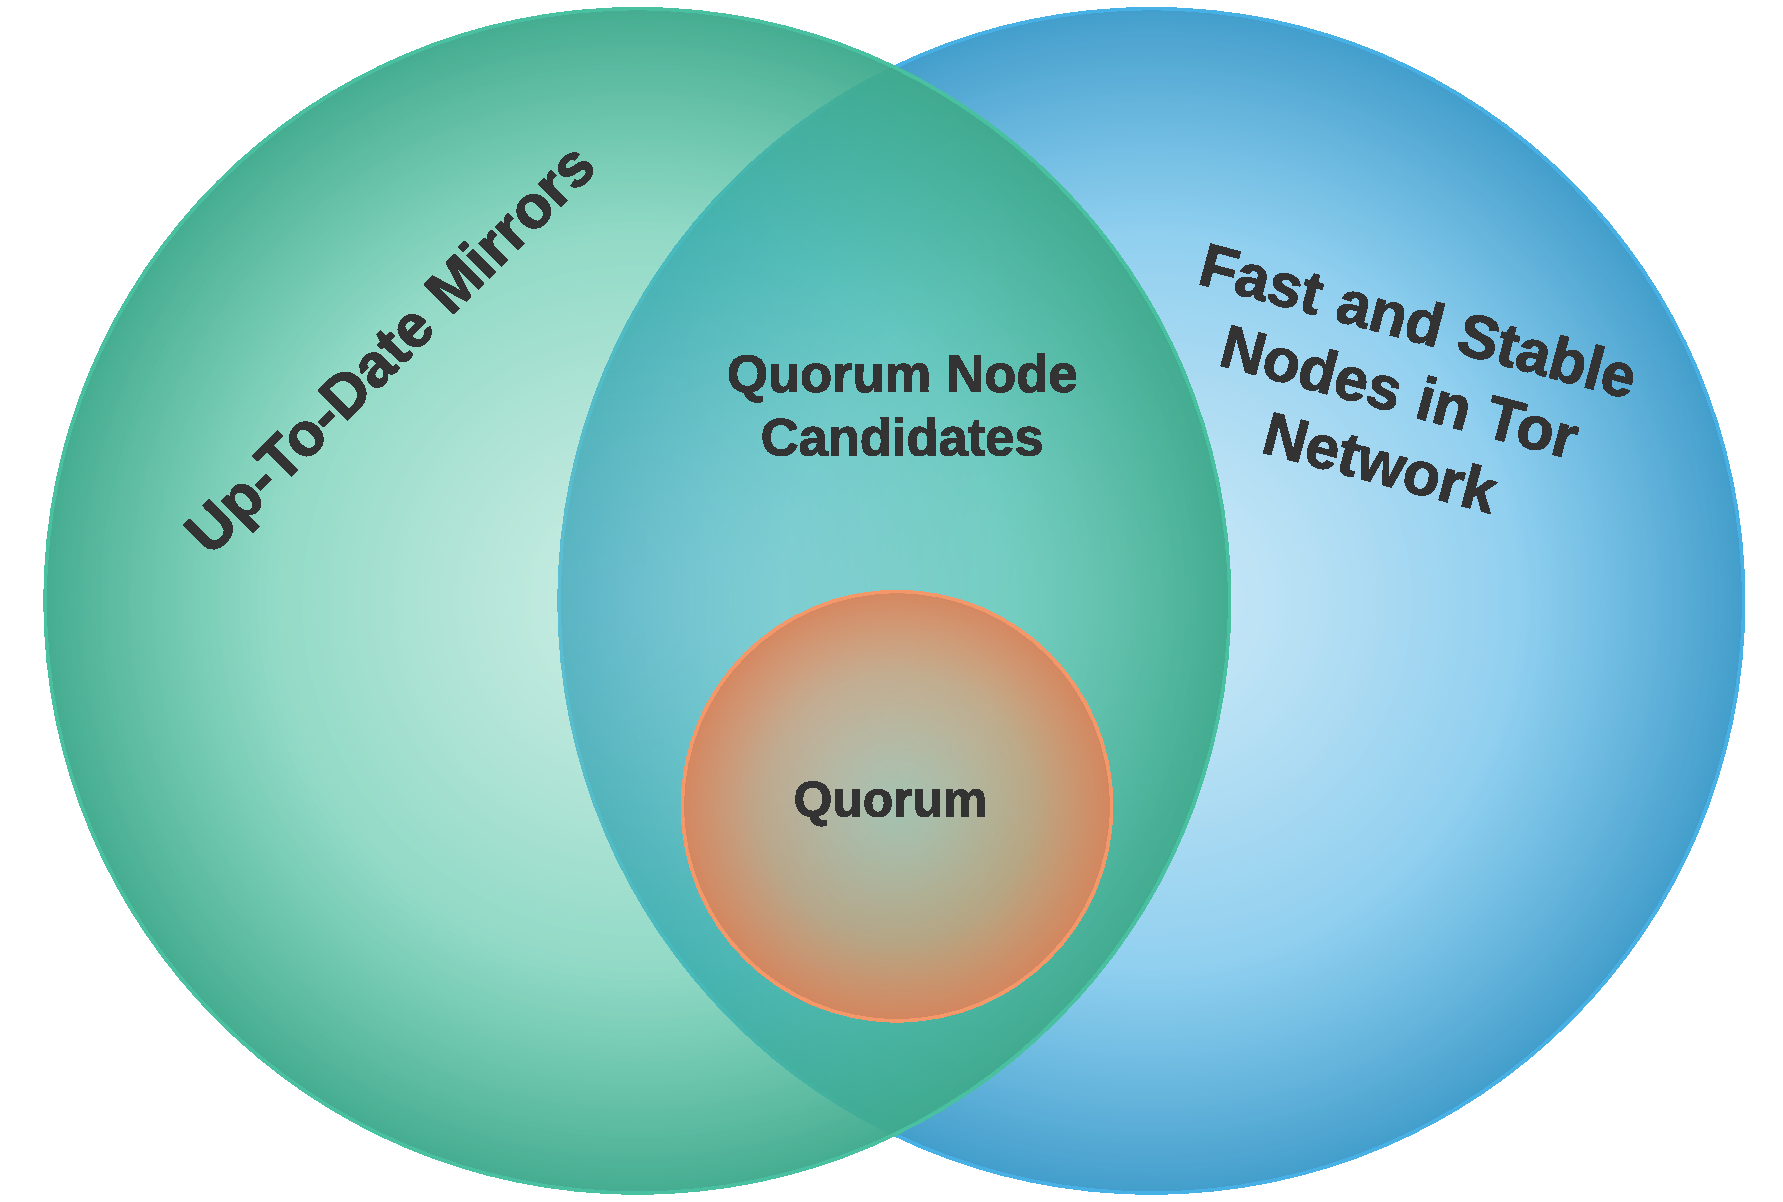
\includegraphics[width=0.5\textwidth]{images/LucidCharts/Participants.pdf}
	\caption{The relationship between Mirrors, Quorum Candidates, and the Quorum. A Mirror is any machine that holds the OnioNS Pagechain, Quorum Candidates are both up-to-date Mirrors and reliable Tor nodes, and the Quorum is randomly selected from the pool of Quorum Candidates.}
\end{figure}

Throughout the rest of this document, let Alice be a Tor client, and Bob be the operator of a hidden service with access to his private HS RSA key. As both Alice and Bob are Tor users, they can obtain and fully verify any past or current set of the three consensus documents described in section \ref{sec:ConsensusDocs}.

\section{Basic Design}
\label{sec:BasicDesign}

\begin{figure}[htbp]
	\centering
	\begin{tikzpicture}[->, node distance=2.4cm, main node/.style={circle, fill=blue!20, draw, font=\sffamily\bfseries}]

			\node[main node] (1) {$ R_{G} $};
			\node[main node] (2) [right of=1] {};
			\node[main node] (3) [right of=2] {Alice};
			\node[main node] (4) [right of=3] {};

			\node[main node] (5) [below of=1] {$ R_{E} $};
			\node[main node] (6) [right of=5] {$ R_{M} $};
			\node[main node] (7) [right of=6] {};
			\node[main node] (8) [right of=7] {};

			\node[main node] (9) [below of=5] {};
			\node[main node] (10) [right of=9] {OnioNS};
			\node[main node] (11) [right of=10] {};
			\node[main node] (12) [right of=11] {$ R_{E} $};

			\node[main node] (13) [below of=9] {};
			\node[main node] (14) [right of=13] {$ R_{M} $};
			\node[main node] (15) [right of=14] {$ R_{G} $};
			\node[main node] (16) [right of=15] {Bob};

			% Alice-OnioNS conversation
			\tikzstyle{EdgeStyle}=[bend right, -, green]
			\Edge[](3)(1)
			\tikzstyle{EdgeStyle}=[bend left=15, -, green]
			\Edge[](1)(6)
			\Edge[](5)(6)
			\draw[thick, ->, red, postaction={decorate, decoration={text along path, text align=center, text={Query}, raise=4pt}}] (5) to [bend left=10] (10){};
			\draw[thick, <-, blue, postaction={decorate, decoration={text along path, text align=center, text={Response}, raise=-9pt}}] (5) to [bend right=10] (10){};

			% Bob-OnioNS conversation
			\tikzstyle{EdgeStyle}=[bend right=15, -, green]
			\Edge[](16)(15)
			\Edge[](15)(14)
			\tikzstyle{EdgeStyle}=[bend left=12, -, green]
			\Edge[](14)(12)
			\draw[thick, red, <-, postaction={decorate, decoration={text along path, text align=center, text={Record}, raise=3pt}}] (10) to [bend left=40] (12){};
			\draw[thick, blue, ->, postaction={decorate, decoration={text along path, text align=center, text={Confirmation}, raise=-10pt}}] (10) to [bend left=30] (12){};

		\end{tikzpicture}
	\caption{Bob uses a Tor circuit to anonymously upload a Record to OnioNS. Alice uses her own Tor circuit to query the system for a domain name, and she is given Bob's Record in response. Then Alice connects to Bob by Tor's hidden service protocol.}
	\label{fig:basicDesign}
\end{figure}

\subsection{Claim on a Domain Name}

To claim a domain name for his hidden service, Bob first generates a valid Record and transmits it over a Tor circuit to a randomly-selected Quorum node. Bob receives a response indicating whether the Record was accepted or not and can confirm that it was re-transmitted by immediately querying another Quorum node for that Record. Mirrors can subscribe to network events from other Mirrors in a peer-to-peer fashion, thus allowing Records and other information to quickly propagate the network, as illustrated in Figure \ref{fig:recordBroadcast}.

\begin{figure}[htbp]
	\centering
	\begin{tikzpicture}[->, node distance=2.2cm, main node/.style={circle, fill=blue!20, draw, font=\sffamily\bfseries}]

			\node[main node] (1) {$ Q_{1} $};
			\node[main node] (2) [right of=1] {$ Q_{2} $};
			\node[main node] (3) [right of=2] {};
			\node[main node] (4) [right of=3] {$ Q_{3} $};

			\node[main node] (5) [below of=1] {};
			\node[main node] (6) [right of=5] {$ Q_{4} $};
			\node[main node] (7) [right of=6] {};
			\node[main node] (8) [right of=7] {};

			\node[main node] (9) [below of=5] {$ R_{M} $};
			\node[main node] (10) [right of=9] {};
			\node[main node] (11) [right of=10] {$ R_{E} $};
			\node[main node] (12) [right of=11] {$ Q_{5} $};

			\node[main node] (13) [below of=9] {};
			\node[main node] (14) [right of=13] {};
			\node[main node] (15) [right of=14] {$ R_{E} $};
			\node[main node] (16) [right of=15] {HS};

			% draw 1st and 2nd part of circuit
			\tikzstyle{EdgeStyle}=[bend right=12, -, green]
			\Edge[](16)(15)
			\Edge[](9)(15)

			% draw last part of circuit
			\tikzstyle{EdgeStyle}=[bend left=17, -, green]
			\Edge[](9)(11)

			% draw record moving from exit to 1st q. node
			\draw[thick, red, <-, postaction={decorate, decoration={text along path, text align=center, text={Record}, raise=3pt}}] (6) to [bend right=15] (11){};

			% draw verification with second q. node
			\draw[thick, red, ->, postaction={decorate}] (12) to [bend left=15] (11){};

			% draw upper left propegation
			\tikzstyle{EdgeStyle}=[bend left=12, ->, blue]
			\Edge[](6)(2)
			\Edge[](6)(1)

			% draw upper right propegation
			\tikzstyle{EdgeStyle}=[bend left=20, ->, blue]
			\Edge[](6)(12)
			\draw[thick, blue] (6) to [bend right=18] (4){};

		\end{tikzpicture}
	\caption{Bob uses his existing circuit (green) to inform Quorum node $ Q_{4} $ of the new Record. $ Q_{4} $ then sends his Record to all other Quorum nodes. Each node stores it in their own Page for long-term storage. Bob confirms from another Quorum node $ Q_{5} $ that his Record has been received.}
	\label{fig:recordBroadcast}
\end{figure}

\subsection{Pagechain Maintenance}

We introduce the Pagechain, a fundamental data structure in OnioNS, in order to keep all participating nodes in synchronization and to save Records in long-term storage. It is a distributed append-only transactional database of a fixed maximum length and is held locally by all Mirrors. Like a blockchain, the Pagechain is designed as a public and fully confirmable data structure -- anyone can confirm the integrity, uniqueness, and validity of all data structures contained within. The head of the chain (the latest Page) is maintained by members of the current Quorum. Assuming that the entire Quorum is honest and maintains perfect communication, all Quorum nodes would be maintaining an identical Page. However, due to malicious modifications or missed communication, disagreements may inevitably form within the Quorum. To avoid these disagreements from misleading the network, we let the network follow the Page maintained by the largest number of Quorum nodes, thus allowing the structure to be partially self-healing as illustrated in Figure \ref{fig:sidechains}.

\begin{figure}[htbp]
	\centering
	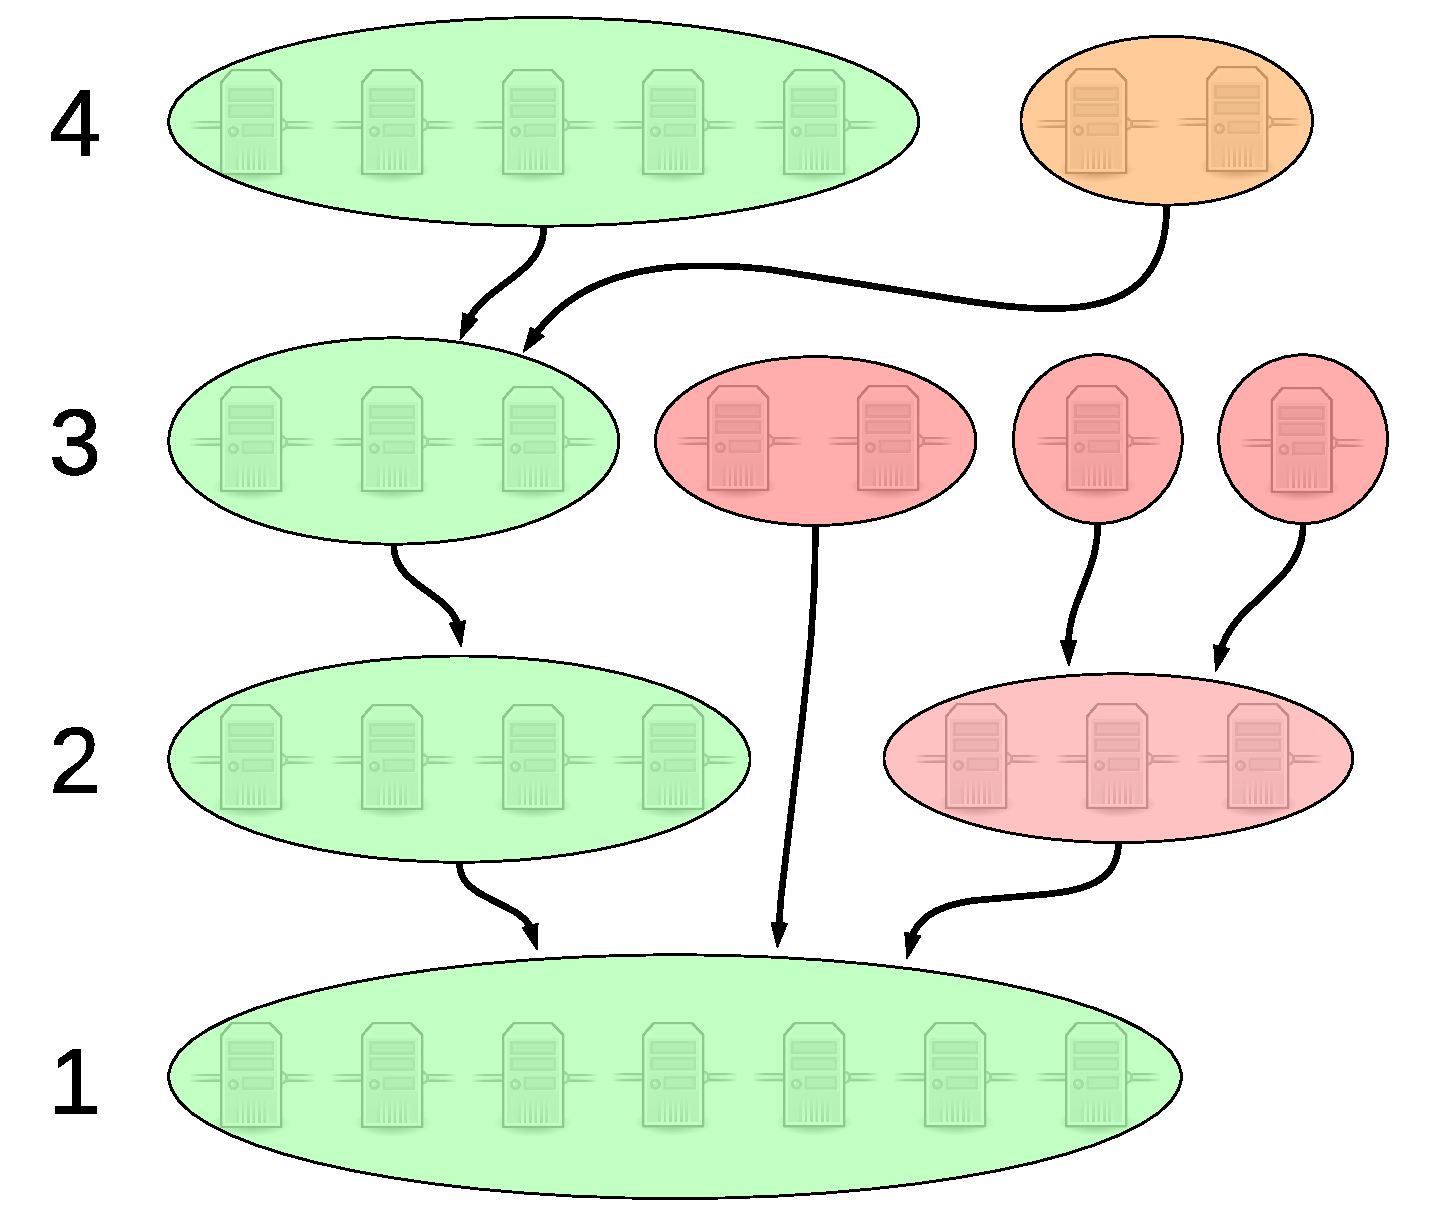
\includegraphics[width=0.55\textwidth]{images/LucidCharts/Page-chain2.pdf}
	\caption{An example Pagechain across four Quorums with three side-chains. $ \mathrm{Quorum}_{1} $ is honest and maintains reliable flooding communication, and thus has identical Pages. Here, red nodes are colluding maliciously, orange missed some communication, and green nodes are acting honestly. Despite the disagreements, across all four days the largest clusters are honest nodes and thus integrity remains in the master Pagechain.}
	\label{fig:sidechains}
\end{figure}

\subsection{Client Request}
\label{sec:ClientRequest}

Typically, Alice will look up a domain name, performing a \emph{domain query}. These are relatively straightforward. Let us assume that Bob, who owns ``onions55e7yam27n.onion,'' has uploaded a Record containing ``example.tor'' and that another party Dave has a Record which claims ``example2.tor'' and that contains ``sub.example2.tor'' $ \rightarrow $ ``example.tor.'' Then Alice can query for ``sub.example2.tor.''

Alice's client-side software recognizes the .tor pseudo-TLD and distinguishes requests containing it from normal Internet lookups. Her software directs the request through a Tor circuit to some Mirror, $ O_{r} $. For security and load reasons, Quorum nodes refuse to respond to queries, so Alice cannot ask them. $ O_{r} $ finds ``sub.example2.tor'' and returns Dave's Record. Alice sees the ``sub.example2.tor $ \rightarrow $ example.tor'' association and now queries $ O_{r} $ for ``example.tor'' since that domain is not in Dave's Record. $ O_{r} $ returns Bob's Record and Alice sees that ``example.tor'' is claimed by Bob and can connect to ``onions55e7yam27n.onion'' via the Tor hidden service protocol. She can send her original request of ``sub.example2.tor'' to Bob, allowing Bob's web server to provide specific content based on that hostname.

In this way, Alice can query a name server and load a hidden service by a meaningful name. We suggest optimizations and security enhancements to this protocol in Section \ref{sec:optimizations}.

\section{Primitives}

\subsection{Cryptographic}
\label{sec:CryptoPrim}

OnionNS makes use of cryptographic hash algorithms, digital signatures, proof-of-work, and a pseudorandom number generator. We require that Tor routers generate an Ed25519\cite{bernstein2011high} keypair and distribute the public key via the consensus document. We note that while we can theoretically use existing NTor keys for digital signatures as it is possible to convert Curve25519 to Ed25519 in constant time, we refrain from this because it is likely not a cryptographically secure operation. Therefore we require Tor to introduce Ed25519 keys to all Tor routers. If this is infeasible, Ed25519 can be substituted with RSA in all instances.

\begin{itemize}
	\item Let $ H(x) $ be a cryptographic hash function. In our reference implementation we define $ H(x) $ as SHA-384.
	\item Let $ S_{\mathit{RSA}}(m, r) $ be a deterministic RSA digital signature function that accepts a message $ m $ and a private RSA key $ r $ and returns an RSA digital signature. Let $ S_{\mathit{RSA}}(m, r) $ use $ H(x) $ as a digest function on $ m $ in all use cases. In our reference implementation we define $ S_{\mathit{RSA}}(m, r) $ as EMSA PKCS1 1.5.
	\item Let $ V_{\mathit{RSA}}(m, E) $ validate an RSA digital signature by accepting a message $ m $ and a public key $ R $, and return true if and only if the signature is valid.
	\item Let $ S_{\mathit{ed}}(m, e) $ be an Ed25519 digital signature function that accepts a message $ m $ and a private key $ e $ and returns a 64-byte digital signature. Let $ S_{\mathit{ed}}(m, e) $ use $ H(x) $ as a digest function on $ m $ in all use cases.
	\item Let $ V_{\mathit{ed}}(m, E) $ validate an Ed25519 digital signature by accepting a message $ m $ and a public key $ E $, and return true if and only if the signature is valid.
	\item Let $ \mathrm{PoW}(i) $ be a one-way collision-free function that accepts an input key $ k $ and returns a deterministic output. Our reference implementation uses a fixed salt and scrypt, a password-based key derivation function which is notable for its large memory and CPU requirements during its operation. The scrypt function provides significantly greater resistance to custom hardware attacks and massively parallel computation primarily due to its memory requirements. This limits attackers to the same software implementation and asymptotic cost as legitimate users\cite{percival2009stronger}\cite{percival2012scrypt}. We choose scrypt because of these advantages over other key derivation functions such as SHA-256 or PBKDF2. For these reasons scrypt is also common for proof-of-work purposes in some cryptocurrencies such as Litecoin.
	\item Let $ \mathit{R}(s) $ be a pseudorandom number generator that accepts an initial seed $ s $ and returns a list of numerical pseudorandom numbers. We suggest MT19937, commonly known as the Mersenne Twister, which is widely used throughout most programming languages and is well known for its speed, long period, and the high quality of its pseudorandom output\cite{matsumoto1998mersenne}.
\end{itemize}

\subsection{Symbols}

\begin{itemize}
	\item Let $ L_{Q} $ represent size of the Quorum.
	\item Let $ L_{T} $ represent the number of routers in the Tor network.
	\item Let $ L_{P} $ represent the maximum number of Pages in the Pagechain.
	\item Let $ q $ be an Quorum iteration counter.
	\item Let $ \Delta q $ be the lifetime of a Quorum in days: every $ \Delta q $ days $ q $ is incremented by one and a new Quorum is chosen.
\end{itemize}

All textual databases are encoded in JSON. JSON is significantly more compact than XML, but retains readability. Its support of basic primitive types is highly applicable to our needs. Additionally, we consider the JSON format safer than byte-level encoding.

\section{Data Structures}
\label{sec:DataStructures}

\subsection{Record}
\label{sec:Record}

There are five different types of Records: Create, Modify, Move, Renew, and Delete. The latter four Records mimic the format of the Create Record with minor exceptions. In each case, \emph{type} is set to the Record type.

\subsubsection{Create}

A Create Record consists of nine components. Fields that are optional are blank unless specified, and all fields are encoded in base64, except for \emph{nameList} and \emph{timestamp}, which are encoded in standard UTF-8.

\renewcommand{\arraystretch}{1.75} % increase spacing between columns
\begin{center}
    \begin{longtabu}{ | l | c | p{9.5cm} |}
    \hline
    \textbf{Field} & \textbf{Required?} & \textbf{Description} \\
    type & Yes & A textual label containing the type of Record. In this case, \emph{type} is set to ``Create''. \\
    name & Yes & The second-level domain name for this hidden service. \\
    nameList & Yes & An array list of zero or more .tor subdomains and their destinations. Destinations use either .tor or .onion TLDs. \\
    contact & No & Bob's PGP key fingerprint if he has one. Client can use this to contact Bob over encrypted email. \\
    consensusHash & Yes & The hash of the consensus document that generated $ \mathit{Quorum}_{q} $ \\
    nonce & Yes & Four random bytes. \\
   	pow & Yes & 16 bytes that store the output of $ \mathrm{PoW}(i) $. \\
   	recordSig & Yes & The output of $ S_{\mathit{RSA}}(m, r) $ where $ m = \mathit{nameList} \concat \mathit{timestamp} \concat \mathit{consensusHash} \concat \mathit{nonce} \concat \mathit{pow} $ and $ r $ is the hidden service's private RSA key. \\
   	pubHSKey & Yes & Bob's public RSA key. \\
    \hline
    \end{longtabu}
\end{center}

\subsubsection{Modify}

A Modify Record allows an owner to update his registration with updated information. The owner corrects the fields, updates \emph{consensusHash}, revalidates the proof-of-work, and transmits the record. Modify Records have a difficulty of $ \frac{\textrm{difficulty}_{\textrm{Create}}}{4} $. Modify Records also act as Renew Records. 

\subsubsection{Move}

A Move Record is used to transfer ownership of the second-level domain name and all associated subdomains from one hidden service key to another. Move Records must not contain modifications and must contain one additional field: \emph{destPubKey}, the public key of the new owner. In this way, transfers are similar to Namecoin. Move records also have a difficulty of $ \frac{\textrm{difficulty}_{\textrm{Create}}}{4} $.

\subsubsection{Renew}

Second-level domain names (and all associated subdomains) expire every $ L_{P}\Delta q $ days because the Pagechain has a maximum length of $ L_{P} $ Pages. Renew Records must be reissued periodically at least every $ L_{P}\Delta q $ days to ensure continued ownership of the domains contained within them. No modifications to existing domain names can be made in Renew records, and the domain names contained within must already exist in the Pagechain. Similar to the Modify and Move records, Renew records have a difficulty of $ \frac{\textrm{difficulty}_{\textrm{Create}}}{4} $.

\subsubsection{Delete}

A Delete Record is used to relinquish ownership rights over a second-level domain name. This is useful if the operator feels that his private key has been compromised or if he has no further user for his domain. This issuance of this Record immediately triggers a purging of the domain name in the system, making it almost immediately available for others. There is no difficulty associated with Delete records, so they can be issued instantly.

\subsection{Page}

Each page contains five fields.

\textbf{prevHash} $ H(\emph{prevHash} \concat  \emph{recordList} \concat \emph{consensusDocHash}) $ of a previous page.

\textbf{recordList} An array list of Records, sorted in a deterministic manner.

\textbf{consensusDocHash} $ H(\mathit{cd}) $.

\textbf{fingerprint} The Tor fingerprint of the relay maintaining this Page.

\textbf{pageSig} The output of $ S_{\mathit{ed}}(H(\mathit{prevHash} \concat \mathit{recordList} \concat \mathit{consensusDocHash})], e) $ where $ e $ is the router's private Ed25519 key.

\section{Protocols}
\label{sec:Protocols}

In section \ref{sec:ConsensusDocs} we described the three consensus documents that Tor routers and clients have: \emph{cached-certs}, \emph{cached-microdesc-consensus}, and \emph{cached-microdescs}. Throughout this section, let ``consensus documents at time $ X $ and day $ Y $'' specifically refer to these three documents when \emph{valid-after} is set to $ X $ and $ Y $. For protocols that specify a hashing of the consensus documents, let the hash only cover \emph{cached-certs} and \emph{cached-microdesc-consensus}; although a router's descriptor is split between \emph{cached-microdesc-consensus} and \emph{cached-microdescs}, the microdescriptors in \emph{cached-microdesc-consensus} include the SHA-256 hash of the entire descriptor. All parties can obtain these consensus documents from any sources because \emph{cached-certs} contains the signing keys that validate \emph{cached-microdesc-consensus}. In practice, it is often efficient to compress these documents en-masse before transmission: they achieve very high compression ratios under Lempel-Ziv-Markov chain algorithm (LZMA).

\subsection{Hidden Services}
\label{sec:ProtoHiddenServices}

\subsubsection{Record Generation}

As invalid Records will be rejected by the network, Bob must generate a valid Record before broadcast:

\begin{enumerate}
	\item Bob selects the value for \emph{type} based on the desired operation.
	\item Bob selects a second-level domain name for his hidden service and assigns it to \emph{name}.
	\item Bob defines subdomains and their destinations, constructing \emph{nameList}.
	\item Bob provides his PGP key fingerprint in \emph{contact} or leaves it blank if he doesn't have a PGP key or if he chooses not to disclose it. Bob can derive his PGP fingerprint with the ``gpg --fingerprint'' Unix command.
	\item Bob sets \emph{consensusHash} to the output of $ H(x) $, where $ x $ is the consensus documents published at 00:00 GMT on day $ \floor[\big]{\frac{q}{\Delta q}} $.
	\item Bob initially defines \emph{nonce} as four zeros.
	\item Let $ \mathit{central} $ be $\mathit{type} \concat \mathit{nameList} \concat \mathit{contact} \concat \mathit{timestamp} \concat \mathit{consensusHash} \concat \mathit{nonce} $. Bob sets \emph{pow} as $ \mathrm{PoW}(\mathit{central}) $.
	\item Bob sets \emph{recordSig} as the output of $ S_{\mathit{RSA}}(m, r) $ where $ m = \mathit{central} \concat \mathit{pow} $ and $ r $ is Bob's private RSA key.
	\item Bob saves the PKCS.1 DER encoding of his RSA public key in \emph{pubHSKey}.
\end{enumerate}

Bob then must increment \emph{nonce} and reset \emph{pow} and \emph{recordSig} until $ H(\mathit{central} \concat \mathit{pow} \concat \mathit{recordSig}) \leq 2^{\mathit{difficulty}} $ where \emph{difficulty} is a fixed constant that specifies the work difficulty. An example of a completed and valid record is shown in Figure \ref{fig:sampleRecord}.

\begin{figure}
\begin{lstlisting}
	{
		"type": "Create",
		"name": "example.tor",
		"subd": {"sub": "onions55e7yam27n.onion"},
		"contact": "AD97364FC20BEC80",
		"consensusHash": "uU0nuZNNPgilLlLX2n2r+sSE7+N6U4DukIj3rOLvzek=",
		"nonce": "AAAABw==",
		"pow":"iOuFHz+eBoxsxDDuX/torg==",
		"recordSig": "bQCtRgJKvkG1Me1Nb0jB1cjN945vHyunFYesi7ildOrYeeZAZLWhf9 azi7YhgL+V/9edPxlGX8+8AMTmrJp6DMWeBVZegANNDzTxkc//x72w88uenQcff JgEKZ1CyBFT3QxtIJvtsd/Te8Hwd60mnAxDR/42rD1QwhJ6PPoOCtc=",		
		"pubHSKey": "MIGfMA0GCSqGSIb3DQEBAQUAA4GNADCBiQKBgQDaXlifPm7dQkw0b F7tOeEdMT9QGM2xoKRZGkNtI8+qeaqx6eiqynVPuS4DYTbr3NppqG7cykteOJlY jBqcDPeaNIytos8q6qYyNEd3VuV6Mm46SL66BL/fIKMxmPNXLp8LfnY UzcUxtdMetxv64Q1Nh46NX6Z8579AXVue3TuKKwIDAQAB"
	}
	\end{lstlisting}
	\caption{A sample registration record. The textual fields are in UTF-8, while the binary fields are in base64. The structure is encoded in JSON.}
	\label{fig:sampleRecord}
\end{figure}

\subsubsection{Record Validation}

Let Carol be a Tor client or a Mirror that receives a Record from another Mirror.

\begin{enumerate}
	\item Carol checks that the Record contains valid JSON and that \emph{type} is either ``Create'', ``Modify'', ``Move'', ``Renew'', or ``Delete''.
	\item Carol checks that \emph{nameList} is has a length $ \in [1,24] $ and that all subdomains have a second-level domain name of the \emph{name} field. Additionally, Carol checks that there is no domain name nor destination that uses more than 16 names, that is longer than 32 characters, or whose total length is more than 128 characters.
	\item Carol checks that \emph{contact} is either 0, 16, 24, or 32 characters in length, and that \emph{contact} is valid hexadecimal.
	\item Carol checks the validity of \emph{recordSig} against \emph{pubHSKey} and $ \mathit{central} \concat \mathit{pow} $.
	\item Carol obtains the $ \floor[\big]{\frac{q}{\Delta q}} $ 00:00 GMT consensus documents and checks $ H(x) $ on it against \emph{consensusHash}. She also confirms that the consensus documents are no older than $ \mathrm{min}(48, 12 * \Delta q) $.
	\item Carol checks that $ H(\mathit{central} \concat \mathit{pow} \concat \mathit{recordSig}) \leq 2^{\mathit{difficulty}} $
	\item Carol calculates $ \mathrm{pow}(\mathit{central}) $ and confirms that the output matches \emph{nonce}.
\end{enumerate}

If at any step an assertion fails, the Record is not valid and Carol does not accept it.

\subsubsection{Record Broadcast}

\begin{enumerate}
	\item Bob derives the current Quorum by the Quorum Derivation protocol.
	\item Bob constructs a circuit, $ c_{1} $, to a Mirror node $ m_{1} $.
	\item Bob asks for and receives from $ c_{1} $ the $ h_{j} = H(\mathit{prevHash} \concat \mathit{recordList} \concat \mathit{consensusDocHash}) $ hash and \emph{pageSig} (the Ed25519 signature on that hash) from each Quorum node.
	\item Bob confirms that $ V_{\mathit{ed}}(h_{j}, E) $ returns true for each $ h_{j} $ and defines $ U $ as the largest set of Quorum nodes that have the same hash.
	\item Bob randomly chooses a node $ n_{1} $ from $ U $ and builds a circuit to it, $ c_{2} $.
	\item Bob uploads his Record through $ c_{2} $ to $ n_{1} $.
	\item Bob uses $ c_{1} $ to ask $ m_{1} $ for his second-level domain name.
	\item Bob has confirmation that his Record was accepted and processed by the Quorum if $ m_{1} $ returns the Record he uploaded.
\end{enumerate}

\subsection{OnioNS Servers}
\label{sec:ProtoOnioNServers}

Let Charlie be the name of an OnioNS Mirror. Charlie listens for incoming Records or signatures from one or more other Mirrors.

\subsubsection{Database Initialization}

\begin{enumerate}
	\item Charlie creates an initial Page $ P_{\mathit{curr}} $ and sets the $ P_{\mathit{prevHash}} $ back-reference based on the Page Selection protocol.
	\item Charlie sets \emph{recordList} to an empty array.
	\item Charlie downloads from some remote source the consensus document $ \mathit{cd} $ issued on day $ \floor[\big]{\frac{q}{\Delta q}} $ at 00:00 GMT and authenticates it against the Tor authority public keys.
	\item Charlie sets $ \mathit{consensusDocHash} = H(\mathit{cd}) $.
	\item Charlie sets \emph{fingerprint} to his Tor fingerprint.
	\item Charlie sets $ \mathit{pageSig} = S_{\mathit{ed}}(H(\mathit{prevHash} \concat \mathit{recordList} \concat \mathit{consensusDocHash}), e) $.
\end{enumerate}

\begin{figure}
	\begin{lstlisting}
	{
		"prevHash": 0,
		"recordList": [],
		"consensusDocHash": "uU0nuZNNPgilLlLX2n2r+sSE7+N6U4DukIj3rOLvzek=",
		"fingerprint": "2FC06226AE152FBAB7620BB107CDEF0E70876A7B",
		"pageSig": "KSaOfzrXIZclHFcYxI+3jBwLs943wxVv3npI5ccY/kBEpyXRSopzjo Fs746n0tJqUpdY4Kbe6DBwERaN7ELmSSK9Pu6q8QeKzNAh+QOnKl0fKBN7 fqowjkQ3ktFkR0Vuox9WrrbNTMa4+up0Np52hlbKA3zSRz4fbR9NVlh6uuQ="
	}
	\end{lstlisting}
	\caption{A sample empty Page.}
	\label{fig:emptyPage}
\end{figure}

\subsubsection{Page Selection}

The Page Selection protocol relies on our security assumption that the largest set of Quorum nodes with agreeing and valid Pages are acting honestly. In this protocol, Charlie chooses the Page $ P_{c} $ maintained by that set.

\begin{enumerate}
	\item Charlie calculates the Quorum via the Quorum Derivation protocol.
	\item Charlie obtains the set of Pages maintained by $ \mathit{Quorum}_{q} $.
	\item For each Page,
		\begin{enumerate}
			\item Charlie checks that \emph{prevHash} references some page from the previous Quorum.
			\item Charlie calculates $ h = H(\mathit{prevHash} \concat \mathit{recordList} \concat \mathit{consensusDocHash}) $.
			\item Charlie checks that $ \mathit{fingerprint} $ is a member of $ \mathit{Quorum}_{q} $.
			\item Charlie checks that $ V_{\mathit{ed}}(h, E) $ returns true.
		\end{enumerate}
	\item Charlie sorts the set of Pages by $ h $, and constructs a 2D array of Pages that have the same $ h $.
	\item For each set of Pages with equal $ h $,
		\begin{enumerate}
			\item Charlie checks that $ \mathit{consensusDocHash} = H(\mathit{cd}) $.
			\item Charlie checks each Record in \emph{recordList} via the Record Validation protocol.
		\end{enumerate}
	\item If the validation of a Page fails, Charlie removes it from the equal-$ h $ list.
	\item Let $ P_{c} $ be chosen arbitrarily from the largest set of valid Pages with equal $ h $.
\end{enumerate}

In this way, Charlie need not preform a deep verification of all Pages from $ \mathit{Quorum}_{q} $ in order to choose a Page.

\subsubsection{Pagechain Validation}

Assume that Charlie has obtained a complete Pagechain. Let $ P_{c} $ be an initial empty Page and let $ f(P_{1}, P_{2}, q) $ accept two Pages and return true if $ P_{1} = P_{2} $ or if $ q = 0 $. For each $ q_{i} $ from the oldest available $ q_{j} $ to the most recent $ q_{k} $,

\begin{enumerate}
	\item Charlie chooses a Page $ P_{c2} $ from $ \mathit{Quorum}_{q_{i}} $ via the Page Selection Protocol.
	\item Charlie checks that $ f(P_{c}, P_{c2}, q) $ returns true, otherwise repeats step 1 to choose another Page from the next largest set of Pages that have equal $ h $.
	\item Charlie calculates $ h_{i} = H(\mathit{prevHash} \concat \mathit{recordList} \concat \mathit{consensusDocHash}) $, fields from $ P_{c2} $.
	\item Charlie checks that $ P_{c2} $'s \emph{prevPage} field equals $ h_{i-1} $ or that $ i = j $, otherwise repeats step 1 to choose the Page from the next largest set.
\end{enumerate}

\subsubsection{Synchronization}
\label{sec:Synchronization}

\begin{enumerate}
	\item Charlie randomly selects a Mirror relay, $ R_{j} $.
	\item Charlie downloads $ R_{j} $'s Pagechain and the Pages used by each Quorum member for each Quorum, obtaining a 2D data structure at most $ L_{P} $ Pages long and $ L_{Q} $ Pages wide.
	\item Charlie checks the downloaded Pagechain via the Pagechain Validation protocol. If it does not validate, Charlie picks another Mirror $ R_{k} $, $ k \ne j $, and downloads the invalid Pages from $ R_{k} $.
	\item Charlie randomly selects a Quorum node $ Q_{c} $ and subscribes to Record and signature networking events from it.
	\item When a set of Pages is available from $ Q_{c} $, Charlie follows the Page Selection protocol to choose a Page that becomes the new Pagechain head.
\end{enumerate}

\subsubsection{Quorum Qualification}

The Quorum is the OnioNS most trusted set of authoritative nodes. They have responsibility over the master Pagechain and are responsible for handling incoming Records from hidden service operators. As such, the Quorum must be derived from the most reliable, capable, and trusted Tor nodes and more importantly Quorum nodes must be up-to-date Mirrors. These two requirements are crucial to ensuring the reliability and security of the Quorum.

The first criteria requires Tor nodes to demonstrate that they sufficient capabilities to handle the increase in communication and processing from with OnioNS protocols. Fortunately, Tor's infrastructure already provides a mechanism that can be utilized to demonstrate this requirement; Tor authority nodes assign flags to Tor routers to classify their capabilities, speed, or uptime history: these flags are used for circuit generation and hidden service infrastructure. Let Tor nodes meet the first qualification requirement if they have the Fast, Stable, Running, and Valid flags. As of February 2015, out of the $ \approx $ 7,000 nodes participating in the Tor network, $ \approx $ 5,400 of these node have these flags and complete the second requirement\cite{TorMetrics}.

To demonstrate the second criteria, the na\"{i}ve solution is to simply ask nodes meeting the first criteria for their Page, and then compare the recency of its latest Page against the Pages from the other nodes. However, this solution does not scale well; Tor has $ \approx $ 2.25 million daily users\cite{TorMetrics}: it is infeasible for any single node to handle queries from all of them. Instead, let each Mirror that meets the first criteria perform the following:

\begin{enumerate}
	\item Charlie calculates $ t = H(\mathit{pc} \concat \floor[\big]{\frac{m - 15}{30}}) $ where \emph{pc} is Charlie's Pagechain and $ m $ is the number of minutes elapsed in that day. Tor's consensus documents are published at the top of each hour; we manipulate $ m $ such that $ t $ is consistent at the top of each hour even with at most a 15-minute clock-skew.
	\item Let Charlie convert $ t $ to base64 and truncate to 8 bytes.
	\item Let Charlie include this new $ t $ in the Contact field in his relay descriptor sent to Tor authority nodes.
\end{enumerate}

We suggest placing $ t $ inside a new field within the router descriptor in future work, but our use of the Contact field eases integration with existing Tor infrastructure. The field is a user-defined optional entry that Tor relay operators typically use to list methods of contact such as an email address. OnionNS would not be the first system to embed special information in the Contact field: PGP keys and BTC addresses commonly appear in the field, especially for high-performance routers.

\subsubsection{Record Processing}

A Quorum node $ Q_{j} $ listens for new Records from hidden service operators. When a Record $ r $ is received, $ Q_{j} $

\begin{enumerate}
	\item $ Q_{j} $ rejects $ r $ if the Record is not valid.
	\item $ Q_{j} $ rejects $ r $ if no such hidden service descriptor exists in Tor's distributed hashtable.
	\item $ Q_{j} $ rejects $ r $ if $ Q_{j} $'s Pagechain contains $ \ge 2 $ Create Records containing $ r $'s \emph{pubHSkey}.
	\item If $ r $ is a Create record, $ Q_{j} $ rejects $ r $ if its second-level domain already exists in $ Q_{j} $'s Pagechain.
	\item If $ r $ is a Modify, Move, Renew or Delete Record, $ Q_{j} $ rejects $ r $ if either of the following are true:
		\begin{enumerate}
			\item $ r $'s Create Record was not found in the Pagechain.
			\item $ r $'s \emph{pubHSKey} does not match the latest Record found in the Pagechain under its second-level domain name.
		\end{enumerate}
	\item If $ Q_{j} $ has rejected $ r $, $ Q_{j} $ informs Bob of this outcome and its reason.
	\item If $ Q_{j} $ has not rejected $ r $, $ Q_{j} $ informs Bob that $ r $ was accepted and $ Q_{j} $ merges the Record into its Page.
\end{enumerate}

\subsection{Tor Clients}
\label{sec:ProtoTorClients}

Let Alice be a Tor client. We assume now that Alice has chosen Charlie as her domain resolver and that Charlie is not a member of the current Quorum, since Quorum nodes don't answer queries.

\subsubsection{Quorum Derivation}

\begin{enumerate}
	\item Alice obtains the consensus documents, $ cd $, published on day $ \floor[\big]{\frac{q}{\Delta q}} $ at 00:00 GMT.
	\item Alice scans $ cd $ and constructs a list \emph{qc} of Quorum Candidates of Tor routers that have the Fast, Stable, Running, and Valid flags and that are in the largest set of Tor routers that publish an identical time-based hash, as described in the Quorum Qualification protocol. She can construct \emph{qc} in $ \mathcal{O}(L_{T}) $ time.
	\item Alice constructs $ f = \mathit{R}(H(\mathit{cd}) $.
	\item Alice uses \emph{f} to randomly scramble \emph{qc}.
	\item The first $ \mathrm{min}(\mathrm{size}(\mathit{qc}), L_{Q}) $ routers are the Quorum.
\end{enumerate}

\subsubsection{Domain Query}

The basic design of the Domain Query is relatively straightforward. 

\begin{enumerate}
	\item Alice constructs a Tor circuit to Charlie.
	\item Alice provides a .tor domain name $ d $ into the Tor Browser, which is treated as a special case by her client software.
	\item \label{step:trim} If $ d $'s highest-level name is ``www'', Alice's software transparently removes that name.
	\item \label{step:level} Alice asks Charlie for the most recent Record $ r $ containing $ d $.
	\item Charlie reviews his Pagechain reverse-chronological order until he finds a Record containing $ d $, which he returns to Alice.
	\item Alice validates $ r $ via the Record Validation protocol. If it does not validate, Alice throws an assertion error.
	\item If the destination for $ d $ in $ r $ uses a .tor TLD, $ d $ becomes that destination and Alice jumps back to step \ref{step:trim}.
	\item Otherwise, the destination must have a .onion TLD, which Alice looks up by the Tor hidden service protocol.
	\item Alice checks that $ r $'s \emph{pubHSKey} matches $ r $'s key in Tor's distributed hash table.
	\item Alice sends the original $ d $ to the hidden service.
\end{enumerate}

We supplement this protocol with an additional data structure in section \ref{sec:MerkleTree} as a defence against Record forgeries. It is also possible for Alice to request and the Page $ p $ containing $ r $ and all digital signatures from each Quorum node, allowing Alice to perform width verification as she can see that a large percentage of Quorum nodes maintained $ p $.

Of course, Alice can be certain that the Record $ r $ she receives is authentic and that $ d $ is unique by performing a full Synchronization and obtaining Charlie's Pagechain for herself, but this is impractical in most environments. It cannot be safely assumed that Alice has storage capacity to hold all the Pages in the Pagechain. Additionally, Tor's median circuit speed is often less than 1 MiBs\cite{TorMetrics}, so for convenience data transfer must be minimized. Therefore Alice can simply fetch minimal information and rely on her trust of Charlie and the Quorum.

\subsubsection{Onion Query}

Alice may also issue a reverse-hostname lookup to Charlie to find second-level domains that resolve to a given .onion address. This request is known as an Onion Query. Charlie performs a reverse-chronological search in the Pagechain for Records whose \emph{pubHSKey} hash to Alice's address. We note that all OnioNS domain names will have Forward-Confirmed Reverse DNS match.

\section{Optimizations}
\label{sec:optimizations}

There are several improvements that be made upon the basic design protocols that significantly enhance the performance of Mirrors when responding to Domain or Onion Requests. We also introduce a Merkle Tree to prevent Mirrors from forging Records or falsely claiming non-existence, thus preventing them from being actively malicious in all significant cases.

\subsection{AVL Tree}

An AVL tree is a self-balancing binary search tree with $ \mathcal{O}(\mathrm{log}(n)) $ time for search, insertion, and deletion operations. We suggest that OnioNS mirrors cache all the Records in its local Pagechain in an AVL tree. After the Pagechain is validated, the Mirror iterates through the Pagechain in chronological order and builds an AVL tree. The leaves of the tree are the location of each Record in the Pagechain, while the keys are the Record's \emph{name} field. The Mirror should then update the AVL tree when it receives new Records that were recently sent to Quorum nodes. Create Records trigger an insert operation, Delete Records cause a deletion, and all other Records update a location pointer to the more recent Record. This approach effectively transforms the lookup time of Records for Domain Queries from $ \mathcal{O}(n) $ to $ \mathcal{O}(\mathrm{log}(n)) $ in the average and worst cases.

\subsection{Trie}

We also suggest utilizing a trie (a digital tree) for efficiently structuring .onion addresses and optimizing Onion Query lookups. If each node in the trie is a character in the .onion address, the trie has a branching factor of 32 and a maximum depth of 16. Let the leaves of the trie be the location of the most recent Record in the Pagechain that has that address as a destination. Like the AVL tree, Mirrors must take care to update the trie cache when processing new Records, but this is efficient as trie search, insertion, and deletion all occur in $ \mathcal{O}(1) $.

\subsection{Merkle Tree}
\label{sec:MerkleTree}

A Merkle tree is a hash tree, a special type of binary tree wherein each non-leaf node is the hash of node's children. We introduce the Merkle tree for two purposes: 1) to prove the non-existence of a domain name, and 2) to prove the authenticity of an existing domain name. This first property is a challenge often overlooked in other domain name systems: even if domain names can be authenticated by a client (e.g. OnioNS Records or SSL certificates) a DNS resolver may lie about the non-existence and claim a false negative. In OnioNS, Alice can download the entire Pagechain and confirm for herself, but as we stated earlier this is not practical. Alice could also query another trusted source such as Quorum Candidates, but this approach does not scale well. Instead, a trusted authority (the Quorum) can sign the Merkle tree once.

Merkle trees also allow anyone to verify that a leaf node is part of a given hash tree in $ \mathcal{O}(\mathrm{log}(n)) $ and without requiring knowledge of the entire tree. We utilize these two properties to allow clients to authenticate Records with minimal networking costs in a single query to an untrusted Mirror name server. To our knowledge this represents the first alternative DNS to authenticate denial-of-existence claims on domains en-masse. To achieve this, let each Quorum node

\begin{enumerate}
	\item Construct an array list \emph{arr}.
	\item For each Record $ r $ in the Pagechain, add $ r_{\mathit{name}} \concat H(r) $ to \emph{arr}.
	\item Sort \emph{arr}.
	\item Construct a Merkle tree $ T $ from \emph{arr}.
	\item Generate $ \mathit{sig}_{T} = S_{\mathit{ed}}(t \concat r, e) $ where $ t $ is a timestamp and $ r $ is the root hash of $ T $.
\end{enumerate}

As Records contains all subdomains under a single second-level domains, $ T $ needs only contain $ r_{\mathit{name}} $ to reference all domains in $ r $, which further saves space. Then during a Domain Query Alice may use $ T $ to authenticate a domain $ d $ and verify non-existence for a Record $ r $.

\begin{enumerate}
	\item Alice extracts the second-level name $ c $ from $ d $.
	\item If $ r $ exists, Charlie returns the leaf node containing $ r $ and all the tree nodes from leaf $ r $ to the root and their sibling nodes, so that Alice can verify authenticity of $ r $ by recomputing the root hash and verify that the largest subset of Quorum nodes signed the same root hash.
	\item If Charlie claims non-existence of $ c $, he returns two adjacent leaves $ a $ and $ b $ (and the nodes on their paths and siblings) such that $ a < c < b $, or in the boundary cases that $ a $ is undefined and $ b $ is the left-most leaf or $ b $ is undefined and $ a $ is the right-most leaf.
	\item If either assertion fails, Charlie is dishonest.
\end{enumerate}

The Quorum must regenerate $ T $ every $ \Delta T $ hours to include new Records. Then Alice needs only fetch the signatures on $ T $ at least every $ \Delta T $ hours to ensure that she can authenticate new Records during the Domain Query. Although new Records can traverse the network nearly instantaneously, Alice cannot authenticate or verify denial-of-existence claims on Records newer than $ \Delta T $. Alice must also fetch the $ L_{Q} $ signature from all Quorum nodes and assert that $ T $ is signed by the largest set of nodes maintaining the same Page so as to agree with our last security assumption.




% END OF DOCUMENT, THE BELOW IS SUPPLEMENTAL NOTES AND OLD WRITINGS

% this really could be a Merkle tree, then the top root could be published in the consensus doc

% todo: this works well for names, but how about for Moves?
% records that are less than a day old will have a hard time with the hashtable, but once in a page they are good

% introduce protocol changes like BTC does: set a logic fork at some point in the future

% Chutney simulator

% the flood allows each Quorum node to check agreements, but this shouldn't be used for Page selection, only to know if it missed something

% malicious node could change his own Pagechain locally, but that wouldn't matter because that isn't shared. Only influence would be queries, but that's also partially negated anyway

% Secondly, we describe how this page-chain can be used by the Tor network to power a publicly-verifiable distributed DNS system on top of existing Tor hidden service infrastructure.

% In any fully-connected network where all participants know everyone's public keys, the page-chain becomes publicly confirmable and can be used for distributed DNS.

%Each \emph{quorum} node has its own \emph{page}. If the nodes in $ quorum_{i - 1} $ remain online and our assumption the majority are acting honestly, there will exist sets (``clusters'') of \emph{pages} that have matching \emph{prevHash}, \emph{recordList}, and \emph{consensusDocHash} fields. Let the choice of $ p_{i - 1} $ in $ p_{i} $ be the most recent \emph{page} in the chain chosen by the nodes in the largest such cluster. In the event that $ p_{i - 1} $ or its records to not follow specifications described herein, $ p_{i - 1} $ should be chosen from the second largest cluster, and so on until $ p_{i - 1} $ is chosen from the largest cluster that provides a valid \emph{page}.

% international encodings?

% todo: table label and table reference do not match

%\emph{TODO: specify how difficulty increases to counteract Moore's Law. Also, is the pow even necessary, or can that be regenerated by anyone?}

%% Let the variable \emph{central} consist of all fields except \emph{recordSig} and \emph{pow}. The issuer must then find a \emph{nonce} such that the SHA-384 of \emph{central}, \emph{pow}, and \emph{recordSig} is $ \leq 2^\textrm{difficulty * count} $, where \emph{difficulty} specifies the order of magnitude of the work that must be done and \emph{count} is the number of second-level domain names claimed. For each \emph{nonce}, \emph{pow} and \emph{recordSig} must be regenerated. When the proof-of-work is complete, the valid and complete record is represented in JSON format and is ready for transmission.

%Bob creates a Create record in which she claims "example.tor" as pointing to her hidden service address, exampleruyw6wgve.onion. Bob then spends computational time and RAM finding a \emph{nonce} such that SHA-384 of \emph{central}, \emph{pow}, and \emph{recordSig} is $ \leq 2^\textrm{difficulty * count} $, where \emph{central} consist of all fields in the Create record except \emph{recordSig} and \emph{pow}, and \emph{count} is the number of second-level domains claimed, in this case one. When the proof-of-work is complete, Bob builds a Tor circuit to Carol and sends her the Create record shown in Figure \ref{fig:sampleRecord}. This process is illustrated in Figure \ref{fig:baseCaseFig}.

% cite paper that shows why recycling the entry node is a good idea
% possible that a malicious node could see his transmission, ignore it, then claim it themselves

%The Modify operation renews the ownership of second-level domain names, so a record of the domain name must already exist in the page-chain and be less than $ L $ days old. Once received, \emph{quorum} nodes update the leaf in their AVL trees with the modified record.

%When a quorum node \emph{candidate} $ c_{j} $ becomes a member of the \emph{quorum}, it constructs an empty \emph{page}. If $ i = 0 $ then $ c_{j} $ sets \emph{prevHash} to zeros and generates \emph{nodeFingerprint} and \emph{pageSig}. Otherwise then $ i > 0 $ so \emph{prevHash} is set as the SHA-384 of \emph{prevHash}, \emph{recordList}, and \emph{consensusDocHash} of $ p_{i - 1} $. \emph{recordList} is set as an empty array, and \emph{consensusDocHash} and \emph{nodeFingerprint} are both defined. $ c_{j} $ then signs the preceding fields with its private key, saving the result in \emph{pageSig}. Finally, it constructs a one-hop bidirectional Tor circuit to all other \emph{quorum} nodes. These circuits are used for synchronization and must remain alive for the duration of that \emph{quorum}. Overall this creates $ \frac{M * (M - 1)}{2} $ new TCP/IP links among \emph{quorum} members.

% OnioNS is a distributed system with public data structures; any machine with sufficient storage and bandwidth capacity -- including machines outside the Tor network -- can become a Mirror by obtaining a copy of the Pagechain from OnionNS nodes.

%Let $ i $ be the current day, $ \Delta i $ be the lifetime of the \emph{quorum}, Alice be the machine becoming a \emph{mirror}, and Bob an existing \emph{mirror}.
%
%\begin{enumerate}
%	\item Alice obtains from Bob his $ \min(i,L) $ most recent \emph{pages} in his cached \emph{page}-chain, where $ L $ is the lifetime of records.
%	\item Alice also obtains the SHA-384 hash, $ h_{p} $, of the concatenation of \emph{prevHash}, \emph{recordList}, and \emph{consensusDocHash} for the \emph{page} used by each \emph{quorum} node for all \emph{quorums} between $ i - \min(i,L) $ and $ i $. Note that each $ h_{p} $ is digitally signed by its respective \emph{quorum} node. See section \ref{sec:Broadcast} for details on how this information is available to Bob.
%	\item Alice downloads the $ \frac{\min(i,L)}{\Delta i} $ consensus documents published every $ \Delta i $ days at 00:00 GMT between days $ i - \min(i,L) $ and $ i $. Alice may download these documents from Bob, but to lighten the burden on Bob she may also obtain them from any other source. Bob may have compressed these beforehand to save space: very high compression ratios can be achieved under 7zip.
%	\item The last item that Alice fetches from Bob is the hashtable bitset and the root of the Merkle collision table, which has been signed by all current \emph{quorum} members.
%	\item Starting with the oldest available consensus document and working forward to day $ \floor[\big]{\frac{i}{\Delta i}} $,
%		\begin{enumerate}
%			\item Alice follows the procedures described in section \ref{sec:Quorum} to calculate the old \emph{quorum}.
%			\item She confirms that the oldest \emph{page} she received from Bob is held by the largest cluster of agreeing \emph{quorum} nodes.
%			\item Alice verifies the validity of the \emph{page} and the records contained within it.
%			\item Finally, Alice progresses to the next most recent \emph{page}, repeating the procedure but also verifying that the \emph{prevHash} refers the $ p_{i - 1} $ she was just examining. This process repeats until all $ \min(i,L) $ \emph{pages} have been verified.
%		\end{enumerate}
%	\item Alice extracts all records from the now-validated \emph{page}-chain and constructs the AVL tree and the hashtable bitset with its Merkle tree containing the collisions. As second-level domains expire every $ L $ rotations of the \emph{quorum}, recent Create, Modify, Move, and Renew operations all act as renewals of the domain name and thus are used by Alice to generated these structures. She should process the records in reverse chronological order because a Delete operation causes immediate expiration of an existing domain.
%	\item She confirms that the signatures on the sections of the bitset and the signatures on the Merkle root hash check out against her generated copy. If they do not, Bob may have manipulated the data and she may need to ask someone else.
%	\item Finally, Alice may make the \emph{page}-chain and consensus documents that she downloaded from Bob and the binary hashtable that she constructed available to others. She may also respond to Domain and Onion Queries using the AVL tree. She must perform these actions once Alice becomes a quorum member \emph{candidate}.
%\end{enumerate}

%sets \emph{originTime} to the current time, creates \emph{snapshotSig}, and sets $ snap_{x+1} $ to be the currently active snapshot for collecting new records.
%	\item Define an empty array list $ arr $.
%	\item With each node $ q_{k \ne j} $ in the \emph{quorum} using its existing one-hop Tor circuits,
%		\begin{enumerate}
%			\item Sends its $ snap_{x} $ and $ <pageSig_{q_{j}}, nodeFingerprint_{q_{j}}> $, every $ <pageSig_{q_{k}}, nodeFingerprint_{q_{k}}> $ it has received so far, and its signatures on the sections of the hashtable bitset and on the Merkle tree root to $ q_{k} $.
%			\item Receives $ s_{x, k} $ and $ <pageSig_{q_{k}}, nodeFingerprint_{q_{k}}> $ from $ q_{k} $.
%			\item Archives $ <pageSig_{q_{k}}, nodeFingerprint_{q_{k}}> $ and add any records that did not exist in $ snap_{x} $ to $ arr $.
%		\end{enumerate}
%	\item For any missing $ <pageSig_{q_{k}}, nodeFingerprint_{q_{k}}> $, it asks a random \emph{quorum} member $ q_{i \ne k} $ for $ q_{k} $'s $ pageSig_{q_{k}} $. In this way, it has a list of \emph{page} signatures from all \emph{quorum} nodes.
%	\item Merges $ snap_{x} $ and the records in $ arr $ into its \emph{page} and regenerates \emph{pageSig}.
%	\item Updates its AVL tree, hashtable bitset, and Merkle collision tree, and regenerates the signatures on the bitset and on the Merkle root tree.
%	\item Increments $ x $.
%\end{enumerate}

%Trusted authorities (e.g. the \emph{quorum} of size $ M $) can divide the bitset into $ Q $ sections, digitally sign each section, and digitally sign the root hash of the Merkle tree. This allows a DNS resolver to send a $ \frac{C * n}{Q} $-sized section of the bitset and its digital signatures to the client, rather than sending the entire bitmap, which may be larger than $ \frac{C * n}{Q} $ for some choices of $ C $, $ Q $, and the size of the signatures. The assembly of these signatures is detailed in \ref{sec:Broadcast}.

%When Carol switches to a fresh page she will update her AVL tree, hashtable bitset, and trie. At that point, Alice can query Carol for ``example.com'' and Carol will return Bob's record.

%\begin{figure}[htbp]
%	\centering
%	\begin{tikzpicture}[->, node distance=2.5cm, main node/.style={circle, fill=blue!20, draw, font=\sffamily\bfseries}]
%
%			\node[main node] (1) {$ R_{G} $};
%			\node[main node] (2) [right of=1] {};
%			\node[main node] (3) [right of=2] {Alice};
%			\node[main node] (4) [right of=3] {};
%
%			\node[main node] (5) [below of=1] {$ R_{E} $};
%			\node[main node] (6) [right of=5] {$ R_{M} $};
%			\node[main node] (7) [right of=6] {$ Q_{1} $};
%			\node[main node] (8) [right of=7] {$ Q_{2} $};
%
%			\node[main node] (9) [below of=5] {};
%			\node[main node] (10) [right of=9] {$ m_{1} $};
%			\node[main node] (11) [right of=10] {};
%			\node[main node] (12) [right of=11] {$ R_{E} $};
%
%			\node[main node] (13) [below of=9] {};
%			\node[main node] (14) [right of=13] {$ R_{M} $};
%			\node[main node] (15) [right of=14] {$ R_{E} $};
%			\node[main node] (16) [right of=15] {Bob};
%
%			%http://www.texample.net/tikz/examples/tkz-berge/
%			%http://www.texample.net/tikz/examples/graph/
%
%			\tikzstyle{EdgeStyle}=[bend right, -, green]
%			\Edge[](3)(1)
%			\tikzstyle{EdgeStyle}=[bend left=15, -, green]
%			\Edge[](1)(6)
%			\Edge[](5)(6)
%
%			\draw[thick, <-, blue, postaction={decorate, decoration={text along path, text align=center, text={response}, raise=3pt}}] (5) to [bend right=15] (10){};
%
%			\draw[thick, red, <-, postaction={decorate, decoration={text along path, text align=center, text={sync}, raise=3pt}}] (10) to [bend right=15] (7){};
%
%			\tikzstyle{EdgeStyle}=[bend right=15, -, green]
%			\Edge[](16)(15)
%			\Edge[](15)(14)
%			\tikzstyle{EdgeStyle}=[bend left=10, -, green]
%			\Edge[](14)(12)
%			\draw[thick, blue, postaction={decorate, decoration={text along path, text align=center, text={record}, raise=3pt}}] (12) to [bend left=15] (8){};
%
%			\tikzstyle{EdgeStyle}=[-, gray]
%			\Edge[](7)(8)
%
%		\end{tikzpicture}
%	\caption{The hidden service operator Bob anonymously sends a record to the \emph{quorum} ($ c_{1} $ and $ c_{2} $), informing them about his domain name. A node $ m_{1} $ mirrors the \emph{quorum}, which Alice anonymously queries for Bob's domain name.}
%	\label{fig:bigPicture}
%\end{figure}
